\documentclass[a4paper,11pt,oneside,%twoside to print on the back of pages
headsepline,												% Linie für Kopfzeile
footsepline,												% Linie für Fußzeile
bibtotocnumbered									% numb point literaturverz in inhaltsverz => bibliography=tot ocnumbered
]{scrreprt}
%----------------------------------------------------------------------------------------------------------------------------------------------
% STANDART LIBS
\usepackage[T1]{fontenc}
\usepackage[utf8]{inputenc}
\usepackage[ngerman]{babel}    % Deutsche Sprache in automatisch generiertem

% DRUCKBEREICH: \areaset[BCOR]{textwidth}{textheight} %TODO understand
% BCOR ist "Binding Correction", also wieviel Innenrand verloren geht
% A4 hat 297mm x 210mm
% wenn keine Marginalien, dann ist Breite 15cm vielleicht besser
\areaset[1.5cm]{14cm}{25cm} 
%% Die folgende Zeile sorgt dafür, daß die Fußnoten eingerückt werden,
%% und zwar um 2em (class scrbook).
\deffootnote{2em}{2em}{\textsuperscript{\normalfont\thefootnotemark} }

%----------------------------------------------------------------------------------------------------------------------------------------------
% ADDITIONAL LIBS

% source code include
\usepackage{listings} % -> %TODO use minted

% Wrapping text around figures
\usepackage{wrapfig}  %
% containers for things that cannot be broken over a page -> example table, figure
\usepackage{float}
% provides many ways to customise the captions in floating environments
\usepackage{caption} % http://www.ctex.org/documents/packages/float/caption.pdf
% same for subfigues
\usepackage{subcaption} % hint include subpicture

%% Unterstützung für Graphiken und Farben
\usepackage[pdftex]{graphicx}
\usepackage[pdftex]{color}
%\definecolor{DSblue}{rgb}{0,0,0.9}   % example defining a color

% INDEX/GLOSSARY %TODO
%Defines commands for use with MakeIndex
%\usepackage{makeidx} % -> en.wikibooks.org/wiki/LaTeX/Indexing pctex.com/files/managed/3/3a/makeindx.pdf
%\usepackage[xindy,toc]{glossaries}
\usepackage{acronym} %Abkürzungsverzeichniss

%BIBTEX
%used by biblatex for qutes
\usepackage[babel,german=quotes]{csquotes} % load after inputenc
% cite package -> 1. pdflatex xx.tex 2. biber xx 3. pdflatex xx.tex
\usepackage[style=reading,backend=biber]{biblatex} %TODO check diff cite styles
% loads the bib file
\addbibresource{bachelorBib.bib}


% cross referencing and hyperrefs
\usepackage[                % FIXME explain
   pdftex,                  % Ausgabe-Medium: PDF
   colorlinks=true,         % farbige Links in der Bildschirm-Version?
   pdfstartview=Fit,       % wie soll Acrobat starten?
   linkcolor=black,         % Farbe für Querverweise
   citecolor=black,         % Farbe für Zitierungen
   urlcolor=black,          % Farbe für Links
   bookmarks=true
   ]{hyperref}
% non clickable URL   		
\usepackage{url} %TODO remove if hyperref is better

% TODONOTES -> http://tex.stackexchange.com/questions/9796/how-to-add-todo-notes
\usepackage{lipsum}                     % Dummytext
\usepackage{xargs}                      % Use more than one optional parameter in a new commands
\usepackage[pdftex,dvipsnames]{xcolor}  % Coloured text etc.
% -> www.tex.ac.uk/ctan/macros/latex/contrib/todonotes/todonotes.pdf
\usepackage[colorinlistoftodos,prependcaption,textsize=tiny]{todonotes}
\newcommandx{\unsure}[2][1=]{\todo[linecolor=red,backgroundcolor=red!25,bordercolor=red,#1]{#2}}
\newcommandx{\change}[2][1=]{\todo[linecolor=blue,backgroundcolor=blue!25,bordercolor=blue,#1]{#2}}
\newcommandx{\info}[2][1=]{\todo[linecolor=OliveGreen,backgroundcolor=OliveGreen!25,bordercolor=OliveGreen,#1]{#2}}
\newcommandx{\improvement}[2][1=]{\todo[linecolor=Plum,backgroundcolor=Plum!25,bordercolor=Plum,#1]{#2}}
\newcommandx{\thiswillnotshow}[2][1=]{\todo[disable,#1]{#2}}

% Print graphics
% tikz print graphs: http://www.texample.net/tikz/examples/
% bytefield – Create illustrations for network protocol specifications


%----------------------------------------------------------------------------------------------------------------------------------------------
% ADDITIONAL LIBS TO CHECK

%linien in Tabellen
\usepackage{booktabs}
\usepackage{anysize}
\usepackage[onehalfspacing]{setspace}


% math for matrix and $$
%\usepackage{amsmath}
%\usepackage{amssymb}

%\usepackage{lmodern}

%\usepackage{multido}    % FIXME ???????????
%\usepackage{everysel}   % FIXME ???????????
 
%% besserer Flattersatz: \RaggedRight
\usepackage{ragged2e}

% from exposee
\usepackage{latexsym}         % Fuer recht seltene Zeichen

\usepackage[a4paper,lmargin={2.5cm},rmargin={2.5cm},tmargin={3cm},bmargin={2.5cm}]{geometry}
\usepackage{enumerate}

\newcommand{\HRule}{\rule{\linewidth}{0.5mm}}

\pdfinfo{
	/Title		(Synchronisation von Binärbaum-indexierten, verteilten InMemory-NoSQL-Datenbanken)
	/Subject		(Bachelorarbeit)
	/Author		(Paul Kitt)
}
%----------------------------------------------------------------------------------------------------------------------------------------------
\begin{document}

%TODO set 1,5 zeilenabstand , verdana, schriftgroesse 10
%TODO style titelSeite -> check jonny -> richtliene
%TODO check bewilligten title 
\title{{\bf Bachelorarbeit:} \\ \begin{large}Synchronisation von Binärbaum-indexierten, verteilten
InMemory-NoSQL-Datenbanken\end{large}}
\author{
	Paul Kitt \\
	528516   \\	
	paul.kitt@student.htw-berlin.de	\\
\\
\textbf{Studienort:}	\\
	Hochschule für Technik und Wirtschaft Berlin \\
	Angewandte Informatik (FB4) \\
	\textbf{Betreuer:} \\
	Prof. Dr.-Ing. Hendrik Gärtner, HTW Berlin \\
	Jens-Peter Haack,  SpinningWheel GmbH
}


\maketitle
\begin{titlepage}
	\begin{center}
	
		\begin{figure}[!htb]
		\minipage{0.5\textwidth}
			\begin{center}
		  		
\includegraphics[width=0.5\textwidth]{bilder/htwLogo.jpeg}
			\end{center}
		\endminipage\hfill
	\minipage{0.5\textwidth}
		\begin{center}
	 		
\includegraphics[width=0.5\textwidth]{bilder/Spinning_O_Wheel-200.png}
		\end{center}	
		\endminipage
	\end{figure}
	
	 \vfill
	 \HRule \\[0.4cm]
	    {\bfseries\Large
	        \begin{LARGE}
	        Bachelorarbeit:\\
	        \end{LARGE} 
	        Synchronisation von Binärbaum-indexierten, verteilten
	InMemory-NoSQL-Datenbanken\\
	    }    
	\HRule \\[1.5cm]
	 \vfill
	
	% Author and supervisor
	\begin{minipage}{0.4\textwidth}
		\begin{flushleft} \large
		\textbf{Author:}\\
		Paul Kitt, 528516 \\
		Angewandte Informatik (FB4) \\	
		Hochschule für Technik und Wirtschaft Berlin\\
		paul.kitt@student.htw-berlin.de	\\~\\
		\textbf{Studienort:}	\\
		Hochschule für Technik und Wirtschaft Berlin \\
		Angewandte Informatik (FB4) \\
		\end{flushleft}
	\end{minipage}
	\begin{minipage}{0.4\textwidth}
		\begin{flushright} \large

		\textbf{Betreuer:} \\
		Prof. Dr.-Ing. Hendrik Gärtner, HTW Berlin \\
		Jens-Peter Haack,  SpinningWheel GmbH
		\end{flushright}
	\end{minipage}
	
	
	 \vfill
	\HRule \\
	%\begin{minipage}{0.4\textwidth}
	%\begin{flushleft} \large
	%Datum/Unterschrift des Betreuers
	%\end{flushleft}
	%\end{minipage}
	\begin{minipage}{0.4\textwidth}
		\begin{flushright} \large
	Datum/Unterschrift des Studenten
		\end{flushright}
	\end{minipage}
	
	\vfill
	{\large \today}
	\end{center}
	% Bottom of the page
	
\end{titlepage}
\tableofcontents
\newpage
\todo[inline]{table of table}
\todo[inline]{table of listings}
Abkürzungsverzeichniss:\\
\begin{acronym}[EB-Baum] % option laengest abk def einzuglänge
 \acro{EB-Baum}{Elastische Binär Baum}
 \acrodefplural{EB-Baum}[EB-Bäume]{Elastische Binär Bäume}

\end{acronym}
	%---------------------------------------------------------------------------------------------------------------------------------------------------	
\chapter{Einleitung}
\todo[inline]{Hintergrund, größerer Rahmen, kurze Aufgabenstellung}
 		\begin{enumerate}[1.]
			\item  Problemstellung und Motivation
			\item Zielsetzung
			\item Rahmen und Aufbau der Arbeit
		\end{enumerate}
		
	Mögliche Punkte:
	-> Motivation
	-> Aufgabenbeschreibung
	-> Inhalt und Aufbau der Arbeit	
		
	%---------------------------------------------------------------------------------------------------------------------------------------------------			
\chapter{Grundlagen}
\todo[inline]{	theoretische Grundlagen, Beschreibung von Systemen(nur insoweit, als das diese Grundlagen und Beschreibungen unbedingt für das Verständnis erforderlich sind und nicht als bei studierten Informatikern vorausgesetzt werden kann)}

	\begin{enumerate}[1.]
			\item Grundlagen verwendeter Algorithmen
				\begin{enumerate}[1.]
					\item Binär Bäume
					\item Elastische Binär Bäume
				\end{enumerate}
			\item Definition von Begriffen
				\begin{enumerate}[1.]
					\item Verteilung
					\item Synchronisation
					\item NoSql -> CAP, ACID theoreme die meine db erfüllt 
				\end{enumerate}
			\item Grundlagen Datenbanken (Verteilung, Synchronisation)
				\begin{enumerate}[1.]
					\item MySql
					\item NoSql 
					\item Baumbasierter Indexe
				\end{enumerate}
	\end{enumerate}

\section{Elastische Binär Bäume}
Bei den \enquote{Elastischen Binär Bäumen} handelt es sich um speziell optimierte Variante der \enquote{Binären Suchbäume}. Entwickelt wurden das Konzept von Willy Tarreau\autocite{Tarreau} im Rahmen einer Forschung zum Thema \enquote{Event-scheduling for user-space network applications} und eignen sich daher auch speziell für Betriebssystem Scheduler, bei welchen schnelles priorisieren nach Zeit oder Dringlichkeit wichtig ist. Daten die mit Binär- oder Ganzahlen, wie Integer oder Long, indexiert sind können in dieser wenig bekannten Datenstruktur sehr effizient verwaltet werden. Dabei ist der \enquote{\ac{EB-Baum}} sehr performant wenn es zu sehr vielen den, Baum verändernden, Operationen, wie: Einfügen, Ändern, Abfragen oder Löschen kommt.\unsure{wie richtig zitieren?}\\
Einfügeoperationen und das Abfragen von Blättern wird in O(log n) bewältigt. Löschen in O(1).\\
Als Ausgangskonzepte dienten bei seiner Entwicklung der \enquote{balanciertem Binär Baum}\unsure{mention red black tree} und des \enquote{Radix Baumes}. Da aber Operationen wie Löschen von Blättern bei einem \enquote{balanciertem Binär Baum} O(log n) kosten und der Baum aber gerade Operationen wie diese möglichst schnell bewältigen soll ein signifikanter Nachteil. Bei den \enquote{Radix Bäumen}, die sich laut dem Entwickler Willy Tarreau\autocite[Absatz Introduction]{Tarreau} im Bezug auf Geschwindigkeit sehr gut eigenen, wird aber im Betrieb das allocieren von Speicher und die damit verbundene \enquote{Garbage Collection} zum Perfomanceproblem.\\
Daher ist der \ac{EB-Baum} eine hybride Form aus beiden um diese Mängel aus zu gleichen. Es handelt sich nicht um einen balancierten Baum, was in besonderen Fällen zu einer schlechteren Leistung als die eines \enquote{balanciertem Binär Baum} führt\unsure{mention example}. Die Blätter sind im Baum von links nach rechts aufsteigend, nach einer Binär- oder Ganzahl(e.g. Integer, Long) sortiert.\\
Eine weitere Besonderheit des \ac{EB-Baum} ist dass seine maximale Höhe durch den Datentyp der Schlüssel bestimmt wird.
So kann beispielsweise ein Baum dessen Schlüssel Werte des Datentypes \enquote{Long} sind maximal 64 Ebenen besitzen da der Datentyp aus 64 Bit besteht. Schlüssel werden durch die Abfolge ihrer Binären Repräsentation adressiert.

\subsection{Besonderheiten des Baumes}
Durch die besondere Beschaffenheit des Baumes lassen sich viele Operationen sehr leicht umsetzen wie:
\begin{itemize}
	\item \textbf{Abfragen}
	\begin{itemize}
		\item das Abfragen des ersten und letzten Schlüssels
		\item erlangen des nächst kleineren oder größerem Schlüssel zu einem gegeben Schlüssel
		\item genaues Finden eine Schlüssels
		\item das Finden des ähnlichsten Schlüssels falls dieser nicht enthalten ist
		\item einfaches Abfragen von Bereichen durch ein Prefix
		\item erlangen des vorherigem oder nächstem unterschiedlichen Schlüssel zu einem gegeben Schlüssel
		\item mehrfach auftretende Schlüssel werden immer in ihrer eingefügten Reihenfolge zurück gegeben
	\end{itemize}
	\item \textbf{Einfügen}
	\begin{itemize}
		\item Einfügen mit Duplikaten: Falls ein Werte bereits existiert wird ein Duplikat angelegt
		\item Einfügen von nur einzigartigen Schlüsseln: Falls der Schlüssel vorhanden wird Existierende zurück gegeben
	\end{itemize}
\end{itemize}


\subsection{Aufbau des Baumes}
In dem originalem von Willy Tarreau verfassten Konzept\autocite[Absatz Definitions]{Tarreau} werden die Daten, die Baum hält, in \enquote{EB Knoten}
gespeichert. \enquote{EB Knoten} bestehen aus zwei Teilen:
\begin{itemize}
\item Knoten: verknüpft Blätter sowie anderen Knoten
\item Blatt: ist durch einen Schlüssel adressiert, hält Daten e.g. Referenz auf ein Datenobjekt
\end{itemize}


\begin{wrapfigure}{r}{0.6\textwidth}
  \begin{center}
    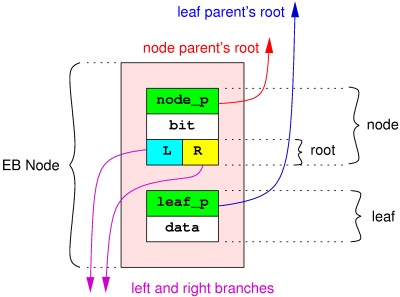
\includegraphics[width=.6\linewidth]{bilder/Ebnode.png}
  \end{center}
 \caption{EB-Knotenelement}
\end{wrapfigure}
Die Aufgabe eines Blattes ist sehr simpel. Es dient nur dazu eingefügte Daten durch einen Pointer zuhalten. Dabei ist es mit einem Schlüssel adressiert und besitzt eine Referenz auf seinen Elternknoten, sowie auf seinen EB-Ursprungsknoten.\\
Ein jedes Knotenelement besteht aus einer Referenz auf sein höher liegenden Elternknoten, dem Ebenenbit \unsure{Darf ich das Bild benutzen?} und zwei Referenzen auf seine Kinderknoten. \\ Das Ebenenbit ist eine Zahl und repräsentiert binär die niedrigste Bitposition des Schlüssels über dem alle Bits gleich sind. Alle unter dem Knoten liegenden Schlüssel haben sich somit bis zu diesem Bit die gleich Bitfolge. Der dritte Teil des Knotens ist die Wurzel die aus zwei Referenzen besteht zu entweder weiteren Knoten oder/sowie Blättern verweist. Da es sich um einen binären Baum handelt repräsentiert je Referenz das linke Bit 0 oder das rechte 1. Nur auf Ebene 0, mit dies repräsentierendem Ebenenbit, kann der Knoten zwei Blätter als Wurzel besitzen, da der Schlüssel sich nur um einen Wert an der letzten, nullten Bitstelle unterscheiden kann.\\
Auch wenn Knoten sich später verschieben können diese nie unterhalb des mit ihnen angefügtem Blattes oder in einen anderen Zweig des Baumes gelangen. Falls es erlaubt ist Duplikate einzufügen werden  Knoten mit negativen Ebenenbits versehen.\\
Eine weitere Besonderheit hier ist dass die Wurzelreferenzen nie unbelegt sind. Nur die Wurzel des Wurzelknoten des Baumes ist hier eine Ausnahme. Wenn seine zwei Wurzeln auf \enquote{null} referenziert ist der Baum leer. Sobald der Baum befüllt wird wächst dieser an seiner linken/\enquote{0-Wurzel}. Die rechte Wurzel referenziert immer auf \enquote{null}. Dadurch lässt sich der der Wurzelknoten einfach erkennen.
Sein Ebenenbit ist die höchste Ebene des Baumes und daher automatisch die binäre Länge des Schlüsseldatentyps, e.g. bei Schlüsseln des Datentyps Long wäre das Ebenenbit 64.\\

\subsection{Einfügen von Daten}
Beim einfügen neuer Datensätze wird jeweils ein Blatt, das die Daten hält, sowie ein Knoten mit dem dass Blatt in Kombination eingefügt wird, eingefügt. Der einzige Fall in dem ein Blatt ohne Knoten angefügt wird ist wenn der Baum leer ist.

Beim Einfügen eines neuen Datensatzes wird ein gesamter \enquote{EB-Knoten} erstellt und an der richtigen Position eingefügt. Werden später weitere Werte gespeichert wird bei deren sortiertem einfügen der Baum umstrukturiert. Dies hat zur Folge dass Knoten und Blatt eines vorher übereinander liegenden \enquote{EB-Knoten} auseinander gezogen werden. Da sie aber noch durch gegenseitige Referenzen\unsure{logisch} verbunden bleiben wird der Baum als elastisch bezeichnet was zum Namen \enquote{\ac{EB-Baum}} führt.\\
Die enge Verknüpfung von Knoten und Blatt ist aber nicht zwingend notwendig. In einer, in Java implementierten, Umsetzung von Spinning Wheel, auf der später in dieser Arbeit eingegangen wird, wird ebenfalls beim Einfügen neuer Daten zu jedem Blatt ein Knoten erstellt aber später wenn der Baum sich verändert ist die Verbindung zwischen Knoten und Blatt nicht mehr nachvollziehbar.


 
	%---------------------------------------------------------------------------------------------------------------------------------------------------	
\chapter{Anforderungsanalyse und Vorgehen}
\todo[inline]{	Bewertung von theoretischen Ansätzen, Konzepten, Methoden, Verfahren; informelle Aufgabenbeschreibung, klar formulierte Zielstellung  }
\begin{enumerate}[1.]
			\item Anwendungsumgebung
			\item Anforderungen und Szenarios
		\end{enumerate}
-> Vortrag

Vorgehen:
-> Eingrenzung auf wenige bestandteile der datenbank(halten uIDs, cID, synchro)
-> Implementierung der Basis Klassen und Funktionalitaeten 
-> Implementierung der Simulations und Evaluations elemente
-> Definieren von Tests und deren Analyse

Technisches Umfeld:
(-> Scala mit Akka)

Anforderungen:
?

Testdesign:
-> Entwurf der Testdaten
-> Testdesign -> test eines use cases
-> Unittests: grobe Funktionstests 

\section{Zielstellung}
-> gesamte Idee testen
-> test wieviel sync ops bei welcher delay und fehlerrate
%---------------------------------------------------------------------------------------------------------------------------------------------------
\chapter{Konzept alias Definition/Entwurf}
\todo[inline]{Definition: formale Darstellung der Anforderung mit Hilfe geeigneter Methoden}
\todo[inline]{Entwurf: Diskussion von Lösungsansätzen, Modellierung der konzipierten Lösung}

		\begin{enumerate}[1.]
			\item Modellierung
			\item Systemarchitektur
		\end{enumerate}
\section{Gesamtaufbau?}

aufteilung komponenten und simulations
\subsection{Programmkomponenten}
 alle grob beschreiben
synchro






\subsection{Simulationskomponenten}	
-> master
-> Kommunikationslayer
-> tree compare: als klasse, nachrichten implementation	
		
\section{Synchronisation}
-> ping synchronisation vs komplett check?
-> delta
-> addressierung des deltas via binärzahl
-> suche nach linkestem unterschied ...
%---------------------------------------------------------------------------------------------------------------------------------------------------
\chapter{Implementierung}
\todo[inline]{Realisierung/Umsetzung, Beschreibung der Implementierung, nicht des Programmcodes}
		\begin{enumerate}[1.]
			\item Umsetzung der Systemarchitektur
			\item Beschreibung und Besonderheiten der Implementierung
		\end{enumerate}

\section{EBTree} % teil gurndlage teil implementation
-> Scala implementierung Aufbauend auf einer spinning wheel optimierten java implementation
-> implementierung ohne verbindung von node und leaf
-> unique keys
-> erweiterung von
-> immer sortiert , Elemente werden nach einem Wert hier cID und uID eingefügt und automatisch nach rechts aufsteigend sortiert
binaerlogik beschreiben

basis operationen:
-> einfügen eines Elementes via binär logik
-> aendern eines elementes 
-> entfernen eines elementes

erweiterung des bauems um node state ids
-> deren berechnung

\subsubsection{TreeActor}
-> haelt 2 bäume für uID udn cID

\subsubsection{Acceslayer}
%---------------------------------------------------------------------------------------------------------------------------------------------------
\chapter{Test}
\todo[inline]{Testarten, Testkriterien, Testumgebung, Testergebnisse}
		\begin{enumerate}[1.]
			\item Testkriterien und Szenarien
			\item Demonstration der Funktionalität
			\item Auswertung der Ergebnisse
		\end{enumerate}
%---------------------------------------------------------------------------------------------------------------------------------------------------		
\chapter{Fazit und Ausblick alias Ergebnis}
\todo[inline]{Zusammenfassung, Bewertung der Ergebnisse, Vergleich mit der Zielstellung, Ausblick}









\newpage
\chapter{LaTex todo Test}

\todo[inline]{The original todo note withouth changed colours.\newline Here's another line.}
Durch neue technische Möglichkeiten, wie große Sensornetze zum erfassen von Messdaten, dem kommenden \glqq Internet der Dinge\grqq  oder neuen Anwendungsfeldern wie \glqq Social Media\grqq , fallen immer größer werdende Datenmengen an und es entstehen immer neue Ansprüche diese zu verarbeiten. Neue Datenbankkonzepte  wie \glqq NoSQL\grqq  oder dem auf \glqq MapReduce\grqq basierendem Hadoop und seine stetigen Weiterentwicklung versuchen neue Wege beim Speichern und Verarbeiten der \glqq Big Data\grqq zu gehen\unsure{Is this correct?}\unsure{I'm unsure about also!}. Grade der Bereich Mobilfunk stellt besondere Anforderungen. Neben dem Bedarf an sehr schnellen Zugriffszeiten beim Lesen und Schreiben muss eine sehr hohe Ausfallsicherheit und Verfügbarkeit gewährleistet werden\change{Change this!}. Zusätzlich ist es wünschenswert zur Verarbeitung der Daten möglichst frei und dynamisch seine Schlüssel wählen zu können\info{This can help me in chapter seven!}.\\
Dabei stoßen sowohl alte SQL basierte als auch neue NoSQL basierte Datenbanksysteme an ihre Grenzen \autocite[preNote:siehe][Seite 1312:postNote]{Schlosser2011}.
Ein weiteres, großes Problem vieler bereits existierender Datenbanksysteme ist die Synchronisation\cite[preNote:siehe][Seite 1312:postNote]{Schlosser2011}. So kommt es beispielsweise bei  Nokia Siemens Networks \glqq One-NDS\grqq, eines der marktführenden Produkte\footcite[preNote:siehe][Seite 1312:postNote]{Schlosser2011}, zu folgender Problemstellung. Veränderungen des Datenbank-Masters werden an den Slave weiter gereicht\improvement{This really needs to be improved!\newline\newline What was I thinking?!}. Fällt dieser aber aus, kann der Master seine Änderungen via \glqq journaling\grqq eine Zeit lang nachvollziehen und den Slave wieder aktualisieren. Fällt dieser zu lange aus, ist dies nicht mehr möglich und ein komplettes Backup muss übertragen werden. Dies darf allerdings nicht länger dauern als das \glqq Vollaufen\grqq des \glqq journalings\grqq des Masters\improvement[inline]{The following section needs to be rewritten!}.\\



\newpage
\listoftodos[Notes]

\newpage
\printbibheading
\printbibliography[type=book,heading=subbibliography,title={Buch Quellen}]
\printbibliography[nottype=book,heading=subbibliography,title={Andere Quellen}]
%\printbibliography[keyword=major,heading=subbibliography,title={Major Sources}] -> add keywords via jabref in the bibFile
%\printbibliography[keyword=minor,heading=subbibliography,title={Minor Sources}]

\chapter{Verzeichnisse}
\todo[inline]{Glossar, Abkürzungen, Abbildungen, Tabellen}

\chapter{Anhang}
\todo[inline]{technische Dokumentation, Benutzerhandbuch, Installationsbeschreibung}

\newpage

\hfil\\\\\\

\begin{LARGE}
\textbf{Eigenständigkeitserklärung}\\\\
\end{LARGE} 
Hiermit versichere ich, dass ich die vorliegende Bachelorarbeit selbstständig und nur
unter Verwendung der angegebenen Quellen und Hilfsmittel verfasst habe. Die Arbeit
wurde bisher in gleicher oder ähnlicher Form keiner anderen Prüfungsbehörde vorgelegt.\\\\\\

\parbox{4cm}{\centering Berlin, 04.02.2014\hrule
\strut \centering\footnotesize Ort, Datum} \hfill\parbox{4cm}{\hrule
\strut \centering\footnotesize Unterschrift}

\end{document}
